\documentclass[10pt]{beamer} %handout in[10pt, handout]
\usepackage[round]{natbib}
\newcommand{\ud}{\,\mathrm{d}}
\newcommand{\vx}{\mathbf{x}}
\usetheme{Copenhagen}
\setbeamertemplate{navigation symbols}{}

\title{Causal Bayesian network exploration of \\ the UK Biobank data}
\subtitle{Week 4 Report}
\author[The Biobank Group]{The Biobank Group}
\institute[ATI]{The Alan Turing Institute}
\date{July 15, 2016}
\begin{document}

%----------- titlepage ----------------------------------------------%
\begin{frame}[plain]
  \titlepage
\end{frame}
%----------- slide --------------------------------------------------%
\begin{frame}[plain]{Overview}
 \frametitle{The UK Biobank Project}
    \tableofcontents
\end{frame}
%----------- Section --------------------------------------------------%
\section{Introduction}
\begin{frame}[plain]{Introduction}

\begin{itemize}

\item The UK Biobank is a major national health resource with the aim of improving prevention, diagnosis, and treatment of a variety of diseases

\item More than 500,000 participants - data collected on a wide array of health and lifestyle variables longitudinally

\item Funding obtained for comprehensive neuro and body imaging of 100,000 of these participants

\item To date, imaging data obtained for 8,000 participants 

\item We have access to nearly 6,000 of these


\end{itemize}


\end{frame}

%----------- Section --------------------------------------------------%

\section{Objectives}
\begin{frame}[plain]{Objectives}
\begin{itemize}
\item In the spirit of the Biobank's objectives of improving prevention, diagnosis and treatment of a variety of diseases, this project aims to determine causal links between modifiable risk factors and their effect on the brain \\

\vspace{0.4cm}

\item Knowledge of such causal links can aid in effective prevention and early detection of diseases

\vspace{0.4cm}


\item This is largely an \emph{exploratory} analysis of the vast Biobank dataset - hopefully, interesting and useful links can be discovered which may point towards and facilitate further research

\end{itemize}
\end{frame}




%----------- slide --------------------------------------------------%
\begin{frame}[plain]{Data Cleaning}
Cleaning the data presents several challenges due to 

\setbeamercovered{transparent}

\onslide<1>{\begin{block}{Nested Questions}
Some questions were asked only of those who answered \emph{other} questions in a specific way!
\end{block}}


\onslide<2>{\begin{block}{Different Variable Encodings}
Many variables have different encodings, e.g. -1=`I don't know' and -3=`prefer not to answer' or -10=`I eat less than one slice of bread per week' 
\end{block}}


\onslide<3>{\begin{block}{Different Variable Types}
Data contain continuous, discrete, ordinal, and nominal variables!
\end{block}}

\onslide<4>{\begin{block}{Multiple Visits for each participant}
Each participant may have provided data on a differing number of follow up visits, each on different dates!
\end{block}}


\end{frame}






%----------- slide --------------------------------------------------%
\begin{frame}[plain]{Nested Questions}
To deal with nested questions, we 
\vspace{0.4cm}

\begin{enumerate}
\item Identified which questions were only asked to some participants, depending on answers given to other questions
\item Chose a reasonable value to to `fill-in' for those who were not asked the question
\end{enumerate}
\vspace{0.4cm}

Example:
`Number of cigarettes previously smoked' is asked only of individuals who indicated that they used to be smokers. Those who never smoked have missing values for this question - we replace these missing values with 0, since they used to smoke 0 cigarettes. 

\end{frame}

\begin{frame}[plain]{Variable Encodings}

To deal with non-sensical variable encodings, we searched through all the variables, noting down 
\vspace{0.4cm}

\begin{enumerate}
\item which values encode something strangely   \\

\item what to replace them with that makes sense numerically \\

\end{enumerate}

\vspace{0.4cm}

Example: 'Amount of bread eaten' is measured in number of slices per week - for some reason the option `less than one slice per week' is encoded as `-10', which does not make much sense numerically. We replace this with zero, since we can just assume that eating less than one slice of bread per week will result in no effects due to bread consumption. 


\end{frame}

\begin{frame}[plain]{Variable Types}
We deal with variable types by 
\vspace{0.3cm}
\begin{enumerate}
\item Switching ordering of levels of nominal variable to make them ordinal where possible
\item make dummy variables for levels of nominal variables if nothing else is possible
\end{enumerate}
\vspace{0.3cm}

Example: The question `type of milk consumed' is nominal, as it contains levels `skimmed milk', `semi-skimmed milk', `soya milk' etc, which do not mean anything numerically. For a case like this, we can re-order the levels to represent amount of fat consumed in cow milk - this way the variable becomes ordinal, as it measure an amount of something. An example of making dummy variables is for a question like vitamin consumption, for which we create dummy variables indicating whether participants consume key vitamin supplements of interest.   

\end{frame}



\begin{frame}[plain]{Multiple Visits for each Participant}

\begin{itemize}
\item We are interested in between-subjects effects and so we do not care about repeated measurements \\

\vspace{0.3cm}

\item We must summarise the information over multiple visits for each variable using one value for each participant \\

\vspace{0.3cm}

\item Various ways to do this:

\vspace{0.3cm}

\begin{enumerate}
\item average values of available visits - results in 20\% missing data
\item take last visit - results in 40\% missing data
\item take visit with least missing values (turns out to be first) -  30\%
\end{enumerate} 

\vspace{0.3cm}

\item -First way mixes time points - not ideal \\ -Second way chooses variables closest to imaging was do	ne - but too much missing data \\ -Third way is a compromise - this is what we chose
\end{itemize}
\end{frame}


\section{Missing Data}
\begin{frame}[plain]{Missing Data}
\begin{itemize}

\item After cleaning the data, we removed all subjects for which there were any neuro-imaging related variables missing, as this is one of the main focuses of this project

\vspace{0.4cm}


\item For these participants, the non neuro-imaging data there were 30\% missing values. A lot of these missing values were due to a specific set of variables that were missing for many individuals - these were largely things like bone density measurements which were either all present or all missing.

\vspace{0.4cm}


\item After removing variables that were missing for over 15\% of participants, the amount of missing data was reduced 3\%.

\end{itemize}

\end{frame}


\begin{frame}[plain]{Reduced Data Set}
\begin{itemize}

\item Aside from exploring the relationships between all variables present, as a first step we are interested in exploring relationships on a hypothesis driven subset of the data. 

\vspace{0.5cm}


\item This reduced data set contained 31 non-imaging variables and the 2501 imaging related variables.

\end{itemize}

\end{frame}



%----------- Section --------------------------------------------------%
\section{Dimension Reduction}
\begin{frame}[plain]{Dimension reduction}
\begin{figure}
\includegraphics[width = 0.8\textwidth]{images/idps-dendro-ave-corr.pdf}
\end{figure}

\end{frame}

%----------- slide --------------------------------------------------%
%----------- Section --------------------------------------------------%
\section{Preliminary Causal Study}

\begin{frame}[plain]{Causal inference -- dependency separation}
Graphical representation of causal relationships of variables
\begin{figure}
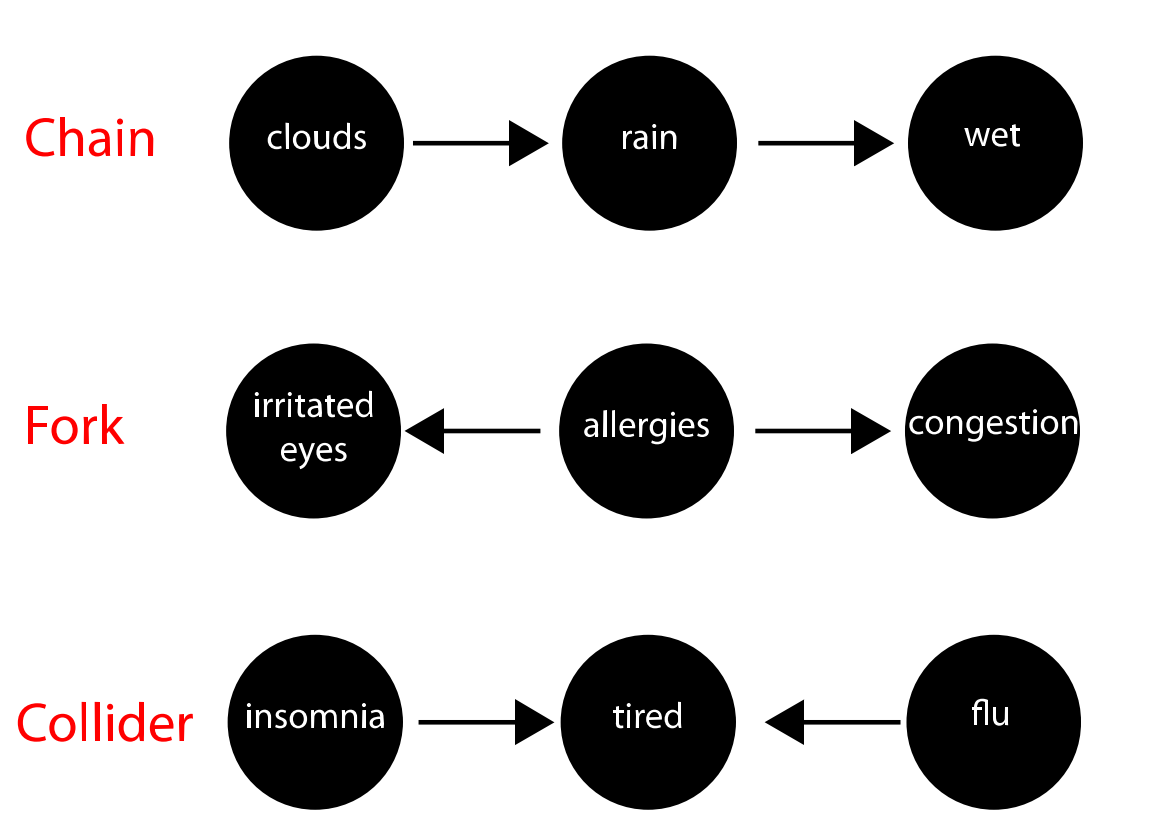
\includegraphics[width = 0.9\textwidth]{images/CIexample.png}
\end{figure}
\end{frame}

%----------- slide --------------------------------------------------%
\begin{frame}[plain]{Bayesian Network}

{\begin{block}{Bayesian Network}
Given a probability distribution $P$ on a set of variables $X$, a Bayesian Network for $(P,X)$ is
\begin{itemize}
\item a DAG (Directed Acyclic Graph) $G$
\item $G$ is a minimal Independence-map of $P$
\end{itemize}
\end{block}}

\begin{figure}
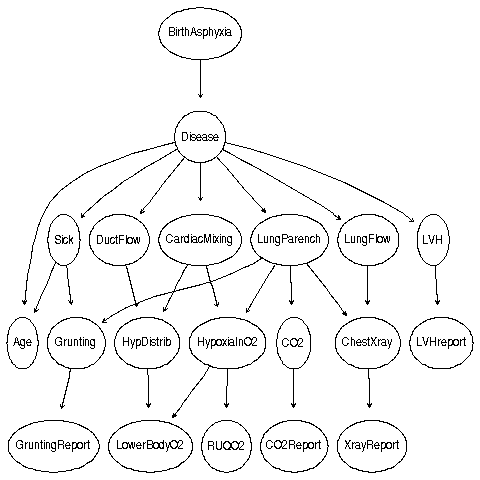
\includegraphics[width = 0.5\textwidth]{images/BNexample.png}
\end{figure}
\end{frame}

%----------- slide --------------------------------------------------%
\begin{frame}[plain]{Causal study using the Bayesian Networks}

\setbeamercovered{transparent}
\onslide<1->{\begin{block}{Causal study of the Biobank data}
\begin{itemize}
\item Represent the joint distribution of the variables by Bayesian networks.
\item Find possible causal relationship from the Bayesian networks.
\end{itemize}
\end{block}}

\onslide<2->{\begin{block}{Learning the Bayes Nets}
\begin{itemize}
\item Structure learning: search the possible graph representations
\begin{itemize}
\item Contraint-based algorithms: Independence tests:  PC
\item Score-based algorithms: greedy search algorithms based on  likelihood, BIC
\end{itemize}

\item Parameter learning
\begin{itemize}
\item More model assuptions and estimate the paramter by maximum likelihood estimation or Bayesian estimation. 
\end{itemize}
\end{itemize}
\end{block}}

\end{frame}

%----------- slide --------------------------------------------------%
\begin{frame}[plain]{A first search}
PC search on a set of hypothesis driven variables -- numerical variables.
\begin{figure}
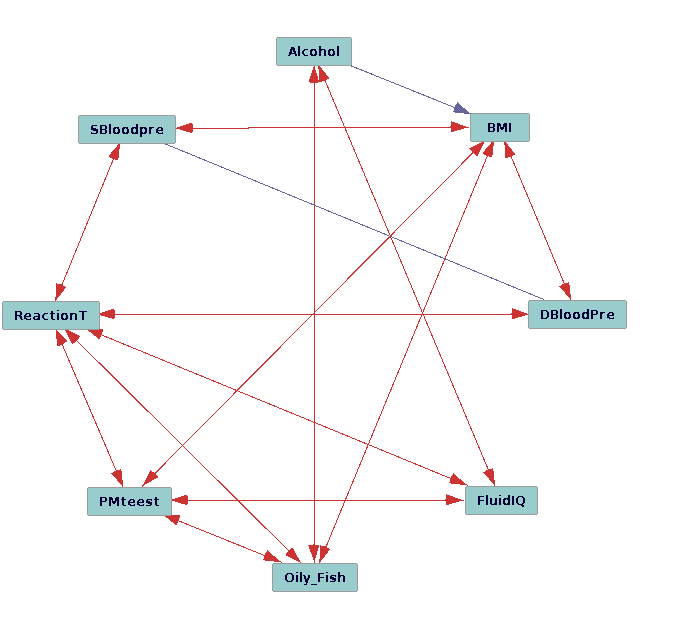
\includegraphics[width = 0.8\textwidth]{images/cont.png}
\end{figure}
\end{frame}

%----------- slide --------------------------------------------------%
\begin{frame}[plain]{A first search}
PC search on a set of hypothesis driven variables -- categorical variables.
\begin{figure}
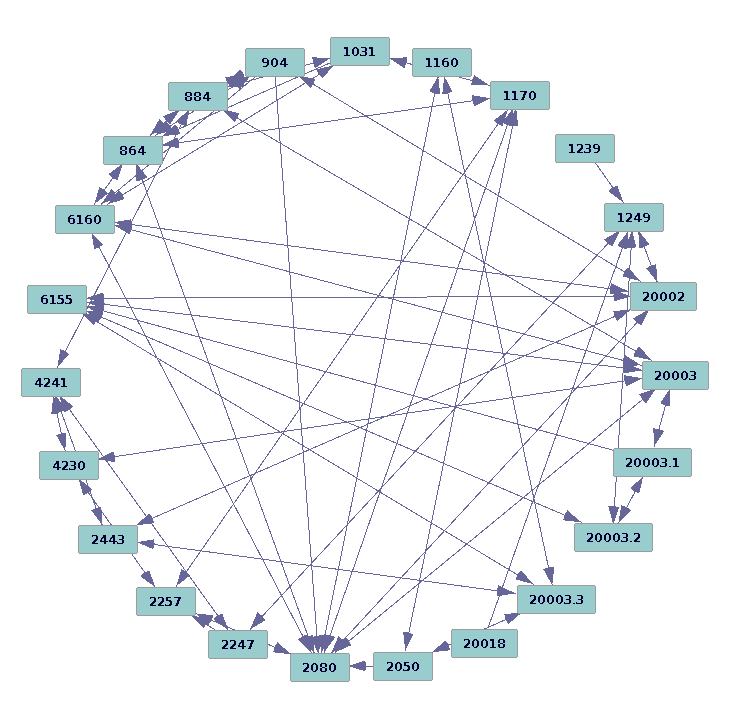
\includegraphics[width = 0.75\textwidth]{images/cat.png}
\end{figure}
\end{frame}

%----------- Section --------------------------------------------------%
%----------- slide --------------------------------------------------%
\section{Next Step}
\begin{frame}[plain]{Next Step}
\begin{itemize}
\item Try causality methods on data set resulting from dimension reduction
\vspace{0.3cm}



\item Work on validation methods to test stability of networks 
\end{itemize}


\end{frame}


\end{document}
